% Software Development for Mobile Devices
\documentclass[11pt,english,numbers=endperiod,parskip=half]{scrartcl}

\usepackage{color}
\usepackage{graphicx}
\usepackage{minted}
\usepackage{fancyhdr}
\usepackage{pdflscape}
\usepackage{listings}
\usepackage{pifont}

\newcommand{\cmark}{\ding{51}}

\pagestyle{fancy}

\rhead{Daniel Parker - 971328X}
\lhead{COS30017 - Software Development for Mobile Devices}

\title{Custom Program}
\subtitle{COS30017 - Software Development for Mobile Devices}
\author{Daniel Parker 971328X}

\date{\today}

\begin{document}
\maketitle
\thispagestyle{empty}

\section{Ideation}
  \subsection{Rationale}
    I would like a way for people to be able to have instant messenger
    conversations around a particular topic whether that be a socially trending
    topic or just people in a common location such as a football game or lecture.

  \subsection{Vision Statement}
    Young adults today are socially active at all times and want to have
    in-depth conversations around a currently trending or popular topic.
    trendChattr is an instant messenger app which allows users to communicate
    based on a currently trending topic on social media or on room local to them.
    Unlike current social media platforms, which are geared towards one person
    stating their opinion and less on the discussion that follows, trendChattr
    will allow for very in-depth and focused discussion around a topic which will
    allow for true and extended input from all users.

  \subsection{Features}
    trendChattr will allow users to register a user handle much like on Twitter
    which they use to login to the app. The users can then select from a list of
    trending topics and local trends those which they would like to chat about
    and chat with other users inside those topics. Users will be able to create
    their own rooms based on their location and will be able to share
    a room on social media for others to get a link to it and join them.

  \subsection{Classification}
    Social

\section{Exploration}
  \subsection{Scenarios}
    \begin{enumerate}
      \item{
        As a social university student, I want to chat to my peers about the
        lecture topic during the lecture without disturbing the class.
      }
      \item{
        As an aspiring politician, I want to have deep discussions with other
        Q\&A viewers during the show's airing.
      }
      \item{
        As a young person, I want to be able to talk to people outside my direct
        social network on certain topics as well.
      }
      \item{
        As a young adventurous urban dweller, I'd like to be able to chat
        to others in the same bar that I'm at so that I can find new friends.
      }
      \item{
        As an avid AFL fan, I would like to be able to chat to others about the
        game while it's being played.
      }
      \item{
        As a news columnist, I would like to be able to create spaces for people
        to chat about the news that I'm reporting and to get their input on the
        issues at hand.
      }
    \end{enumerate}

  \subsection{User Stories}
    \begin{enumerate}
      \item{
        As a user, I would open the app and login but only the first time.
      }
      \item{
        As a user, I would like to see a list of suggested trend chatrooms as
        the main screen.
      }
      \item{
        As a user, I would like to create my own room for my current location or
        another location with a geographic radius of my choice.
      }
      \item{
        As a user, I would like to see the other users usernames in the chatroom.
      }
      \item{
        As a user, I would like to send messages to other users and see both
        mine and their messages in chronological order in the chatroom.
      }
      \item{
        As a user, I would like to be able to register an account upon opening
        the application for the first time.
      }
    \end{enumerate}

  \subsection{Constraints}
    \begin{itemize}
      \item{Chat communication over the internet}
      \item{Login as user (individual login)}
      \item{Custom rooms}
      \item{Rooms based on social trends}
      \item{Room sharing}
      \item{Location based rooms}
    \end{itemize}

  \subsection{UI Designs (Illustrator)}
    \begin{figure}[H]
    \centering{
      \fbox{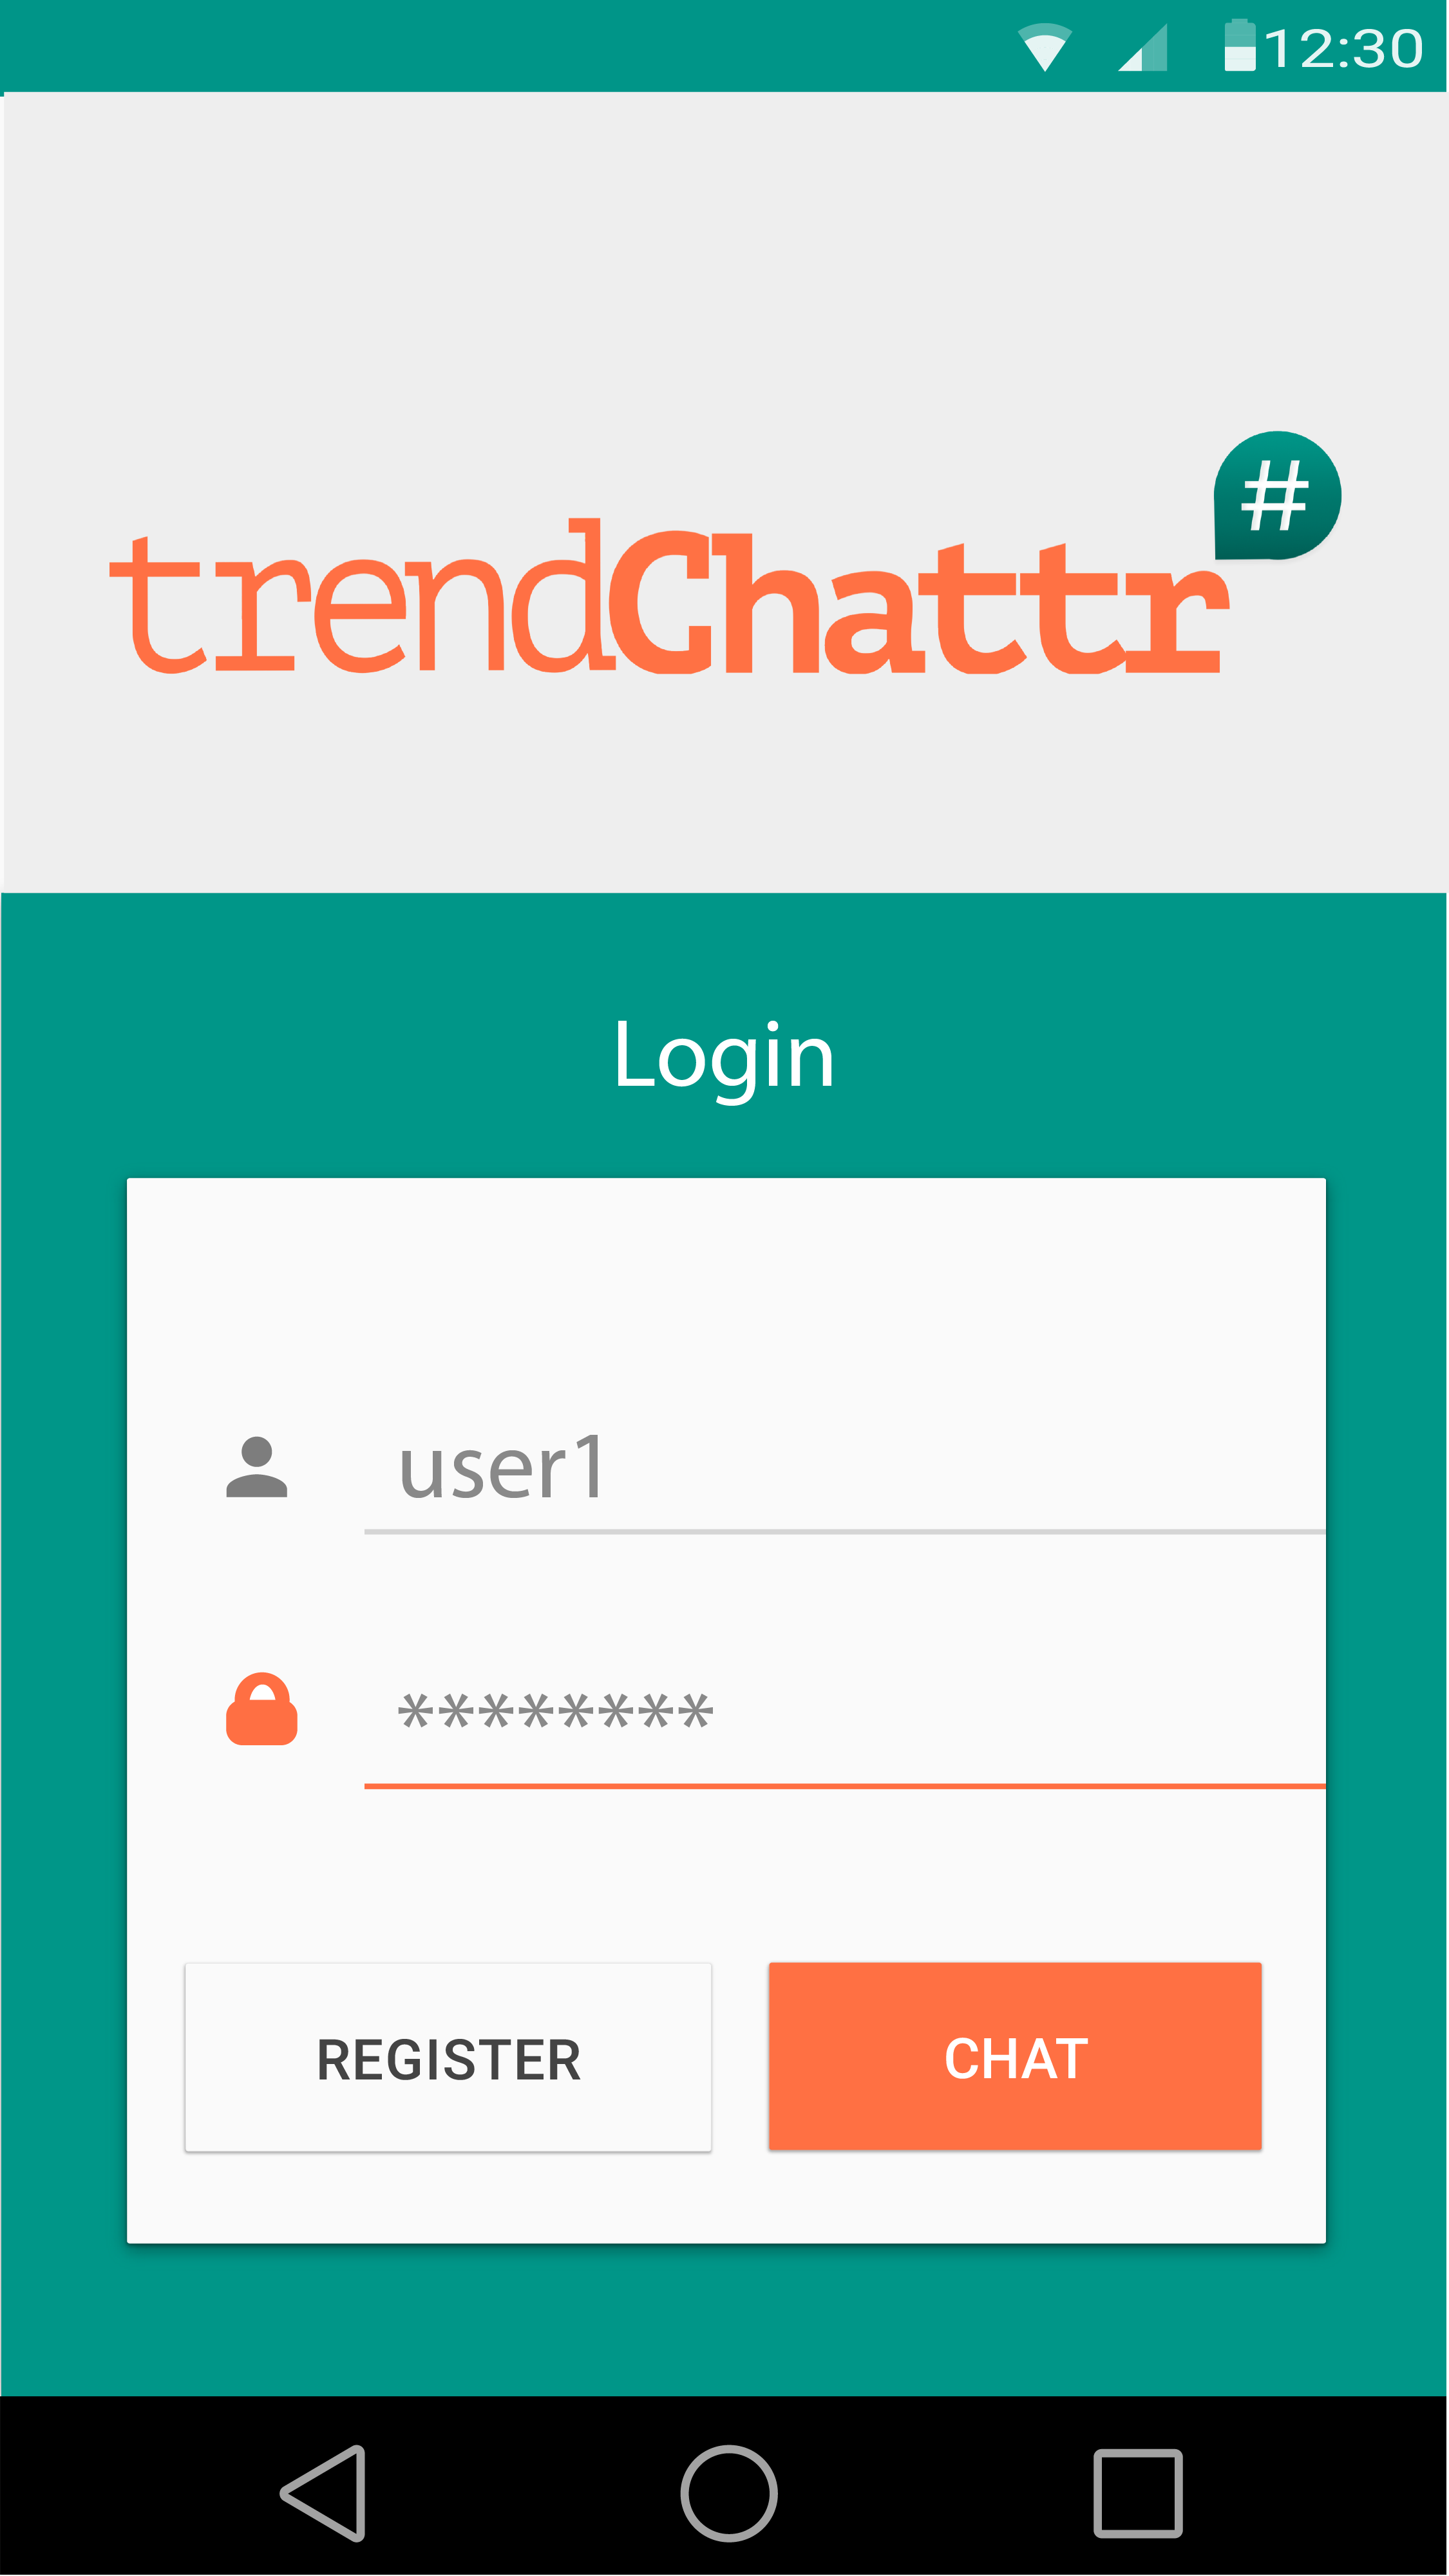
\includegraphics[width=5cm]{images/trendChattr_Login.png}}
    }\\
    \end{figure}
    \begin{figure}[H]
    \centering{
      \fbox{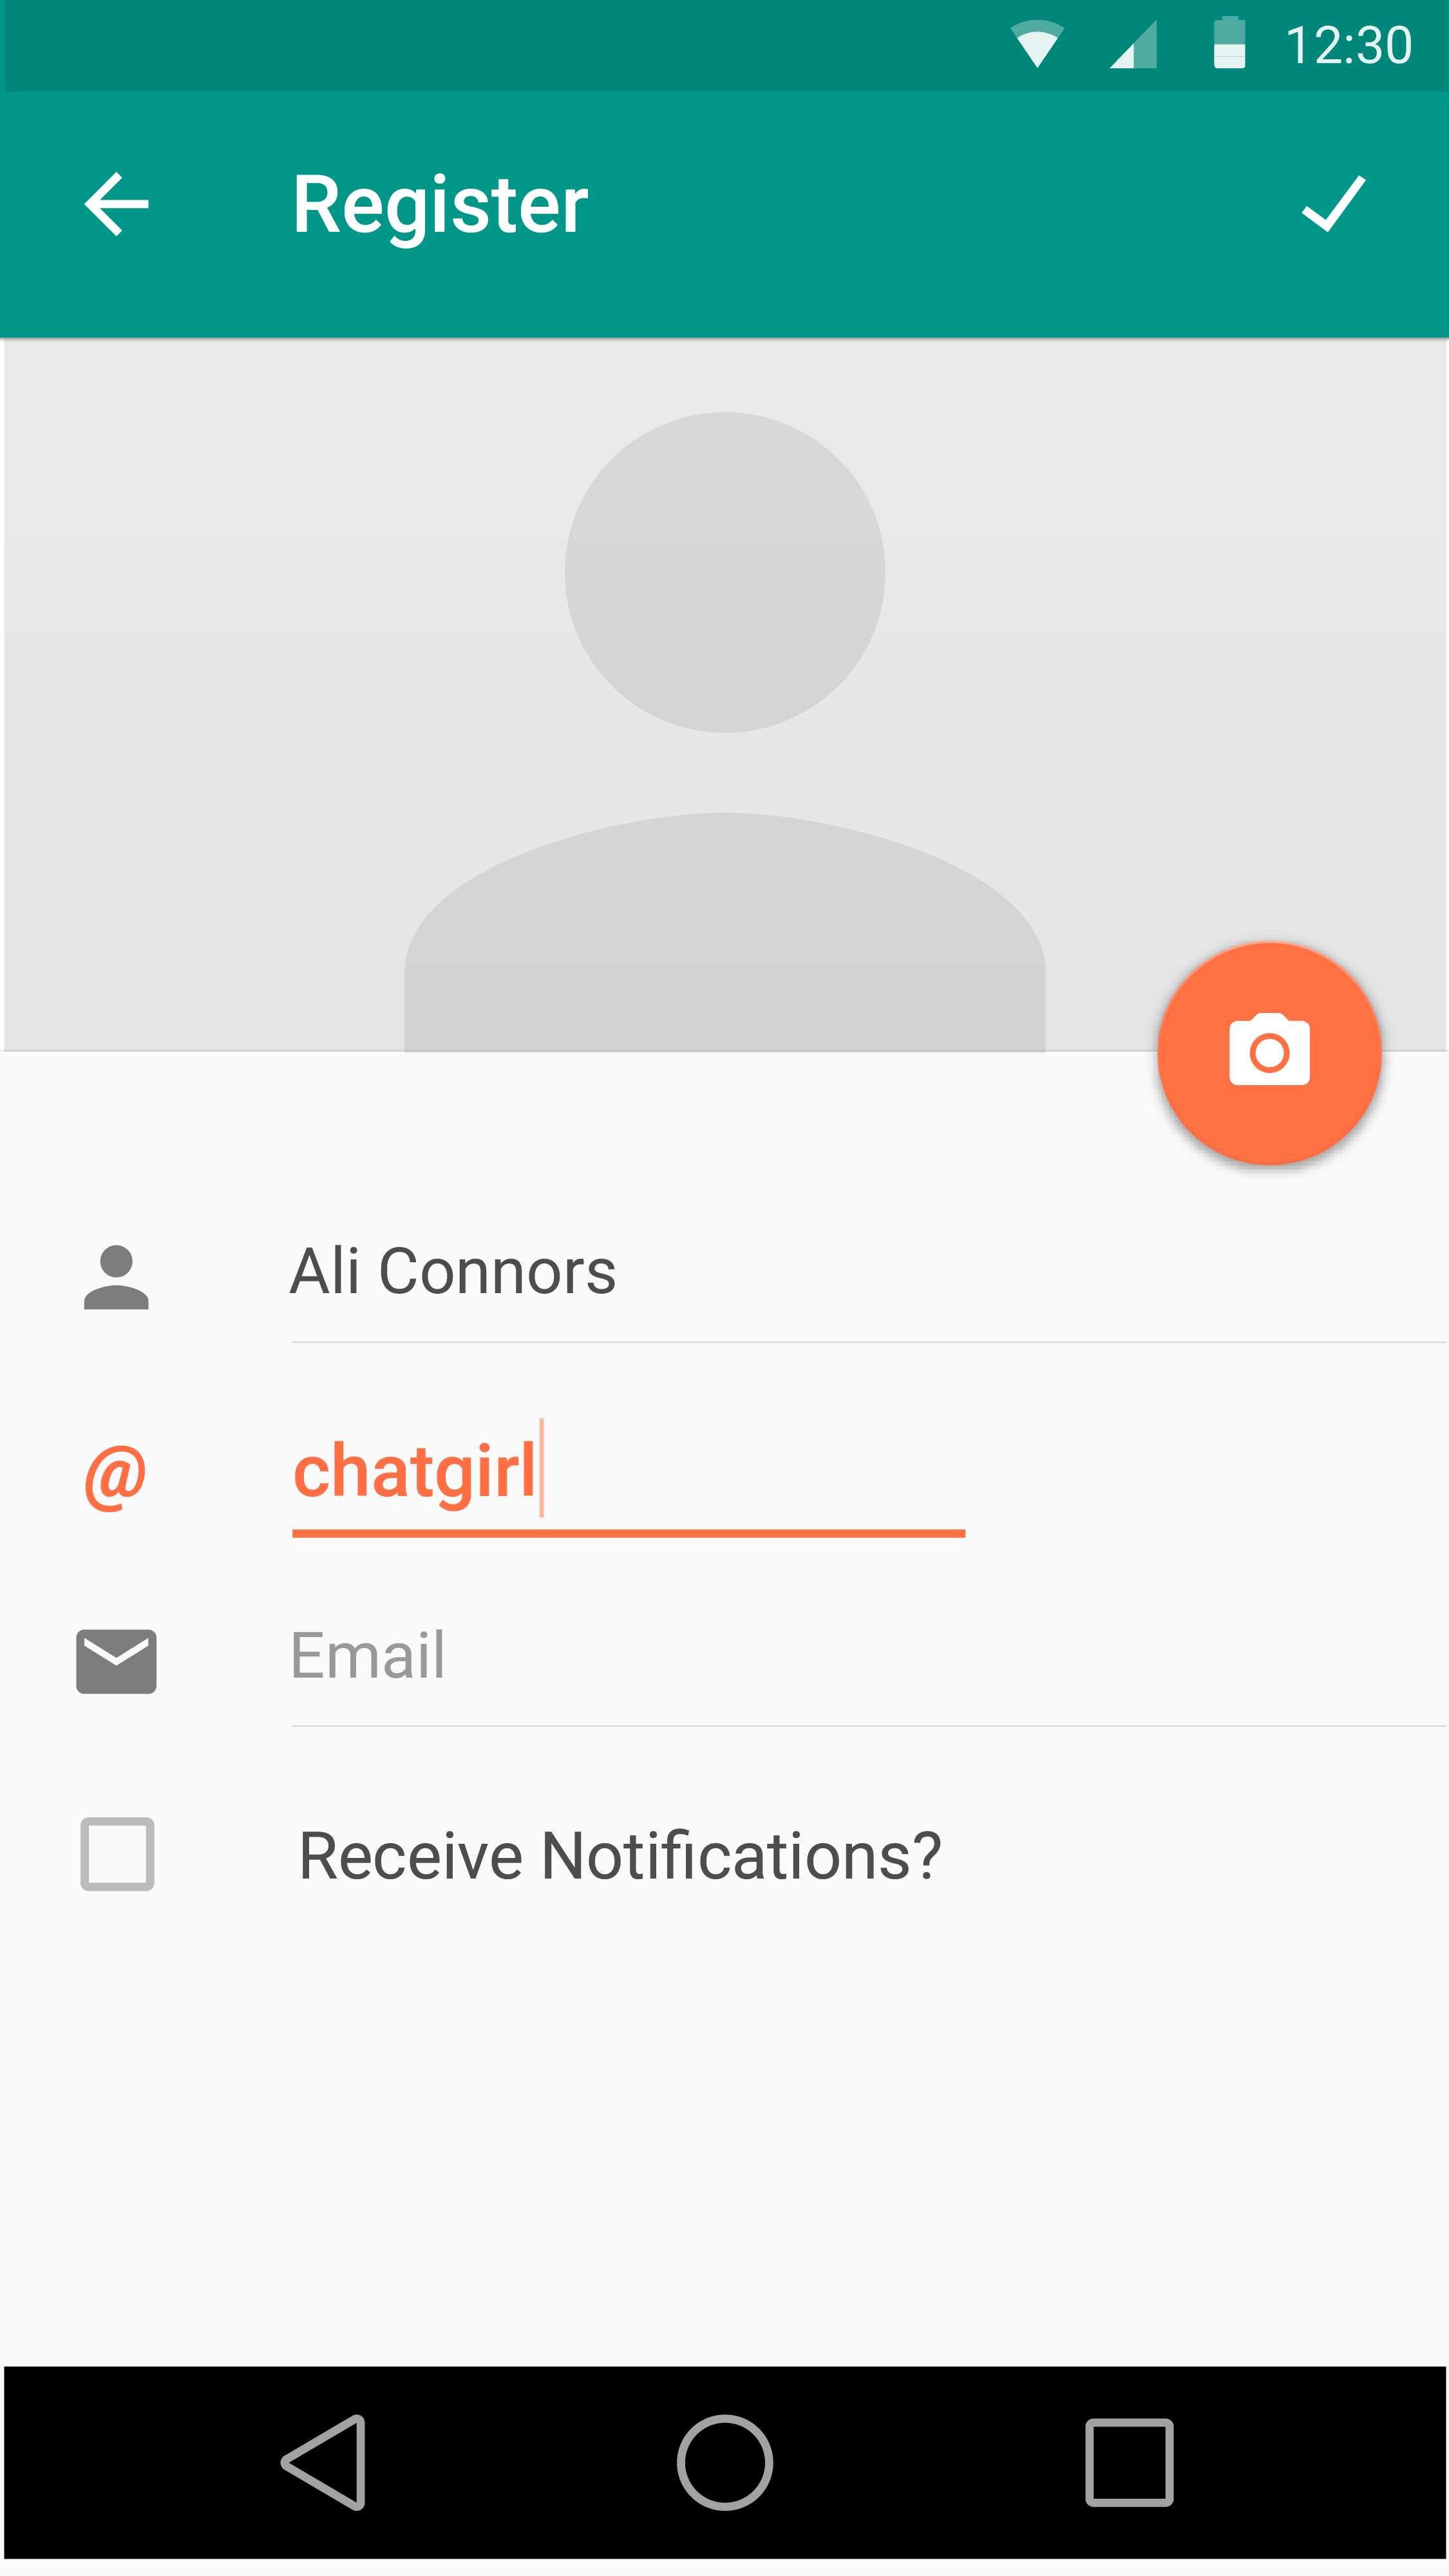
\includegraphics[width=5cm]{images/trendChattr_Register.png}}
    }\\
    \end{figure}
    \begin{figure}[H]
    \centering{
      \fbox{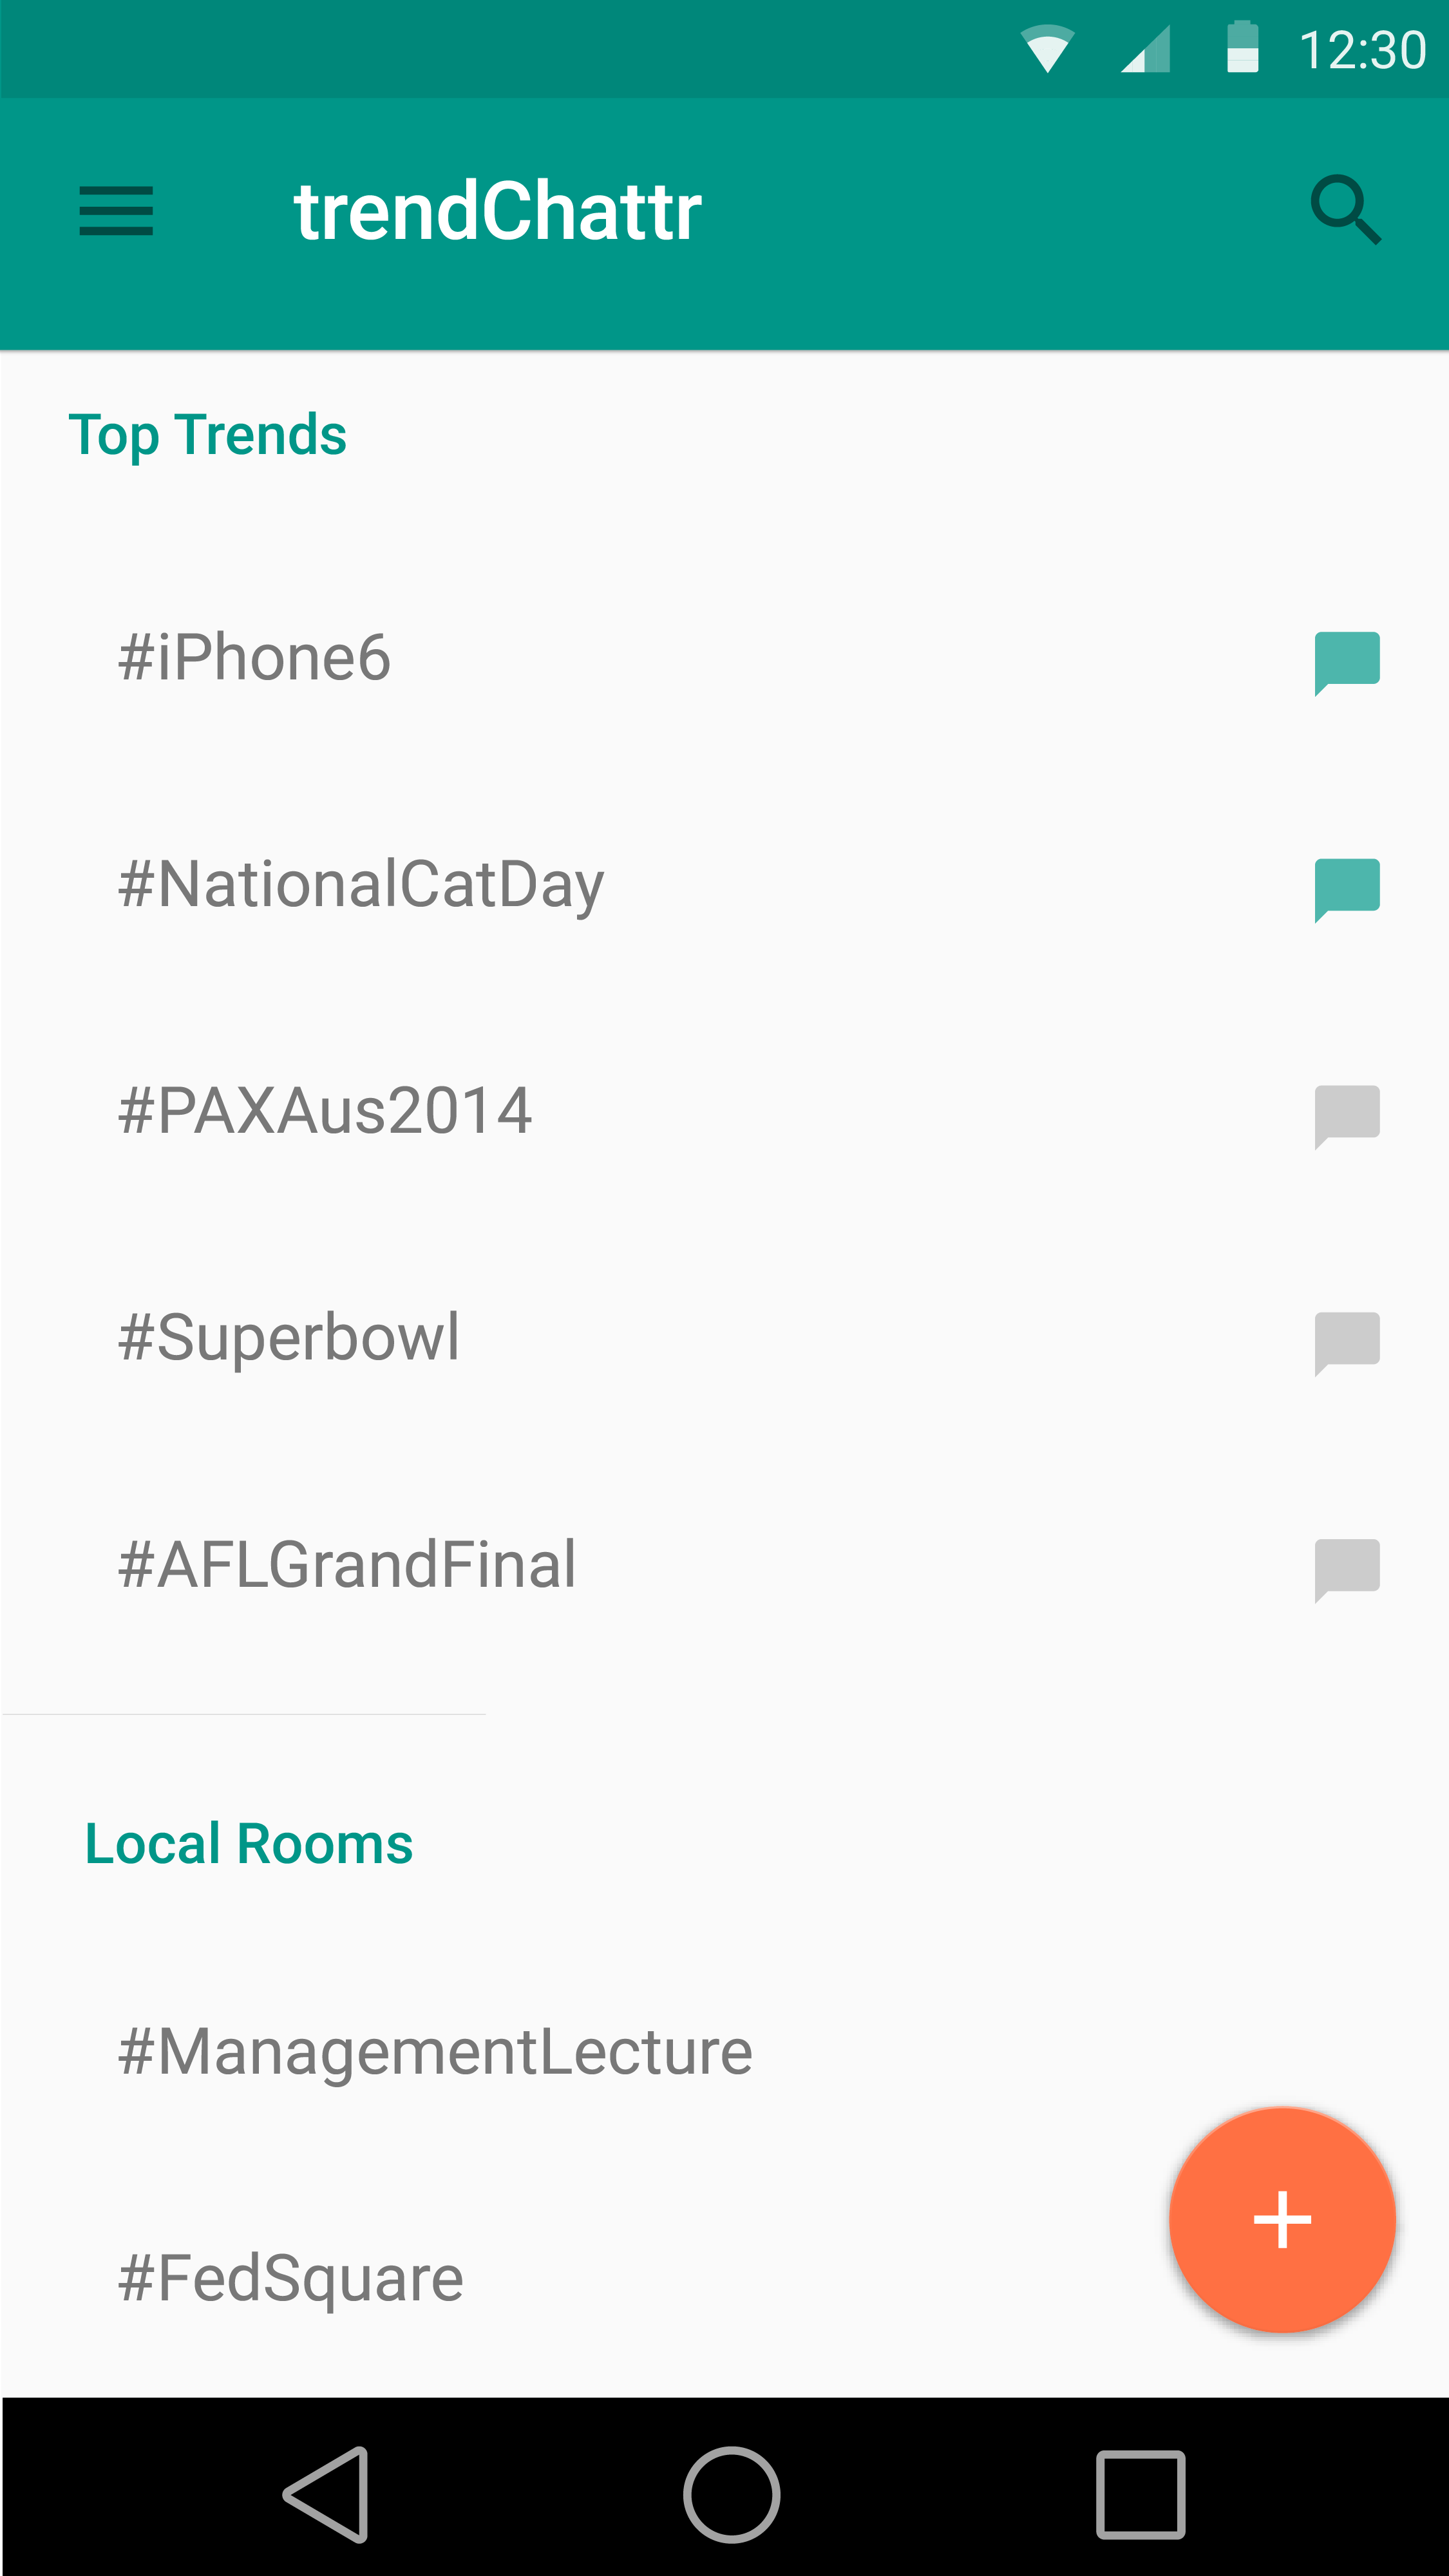
\includegraphics[width=5cm]{images/trendChattr_Trends.png}}
    }\\
    \end{figure}
    \begin{figure}[H]
    \centering{
      \fbox{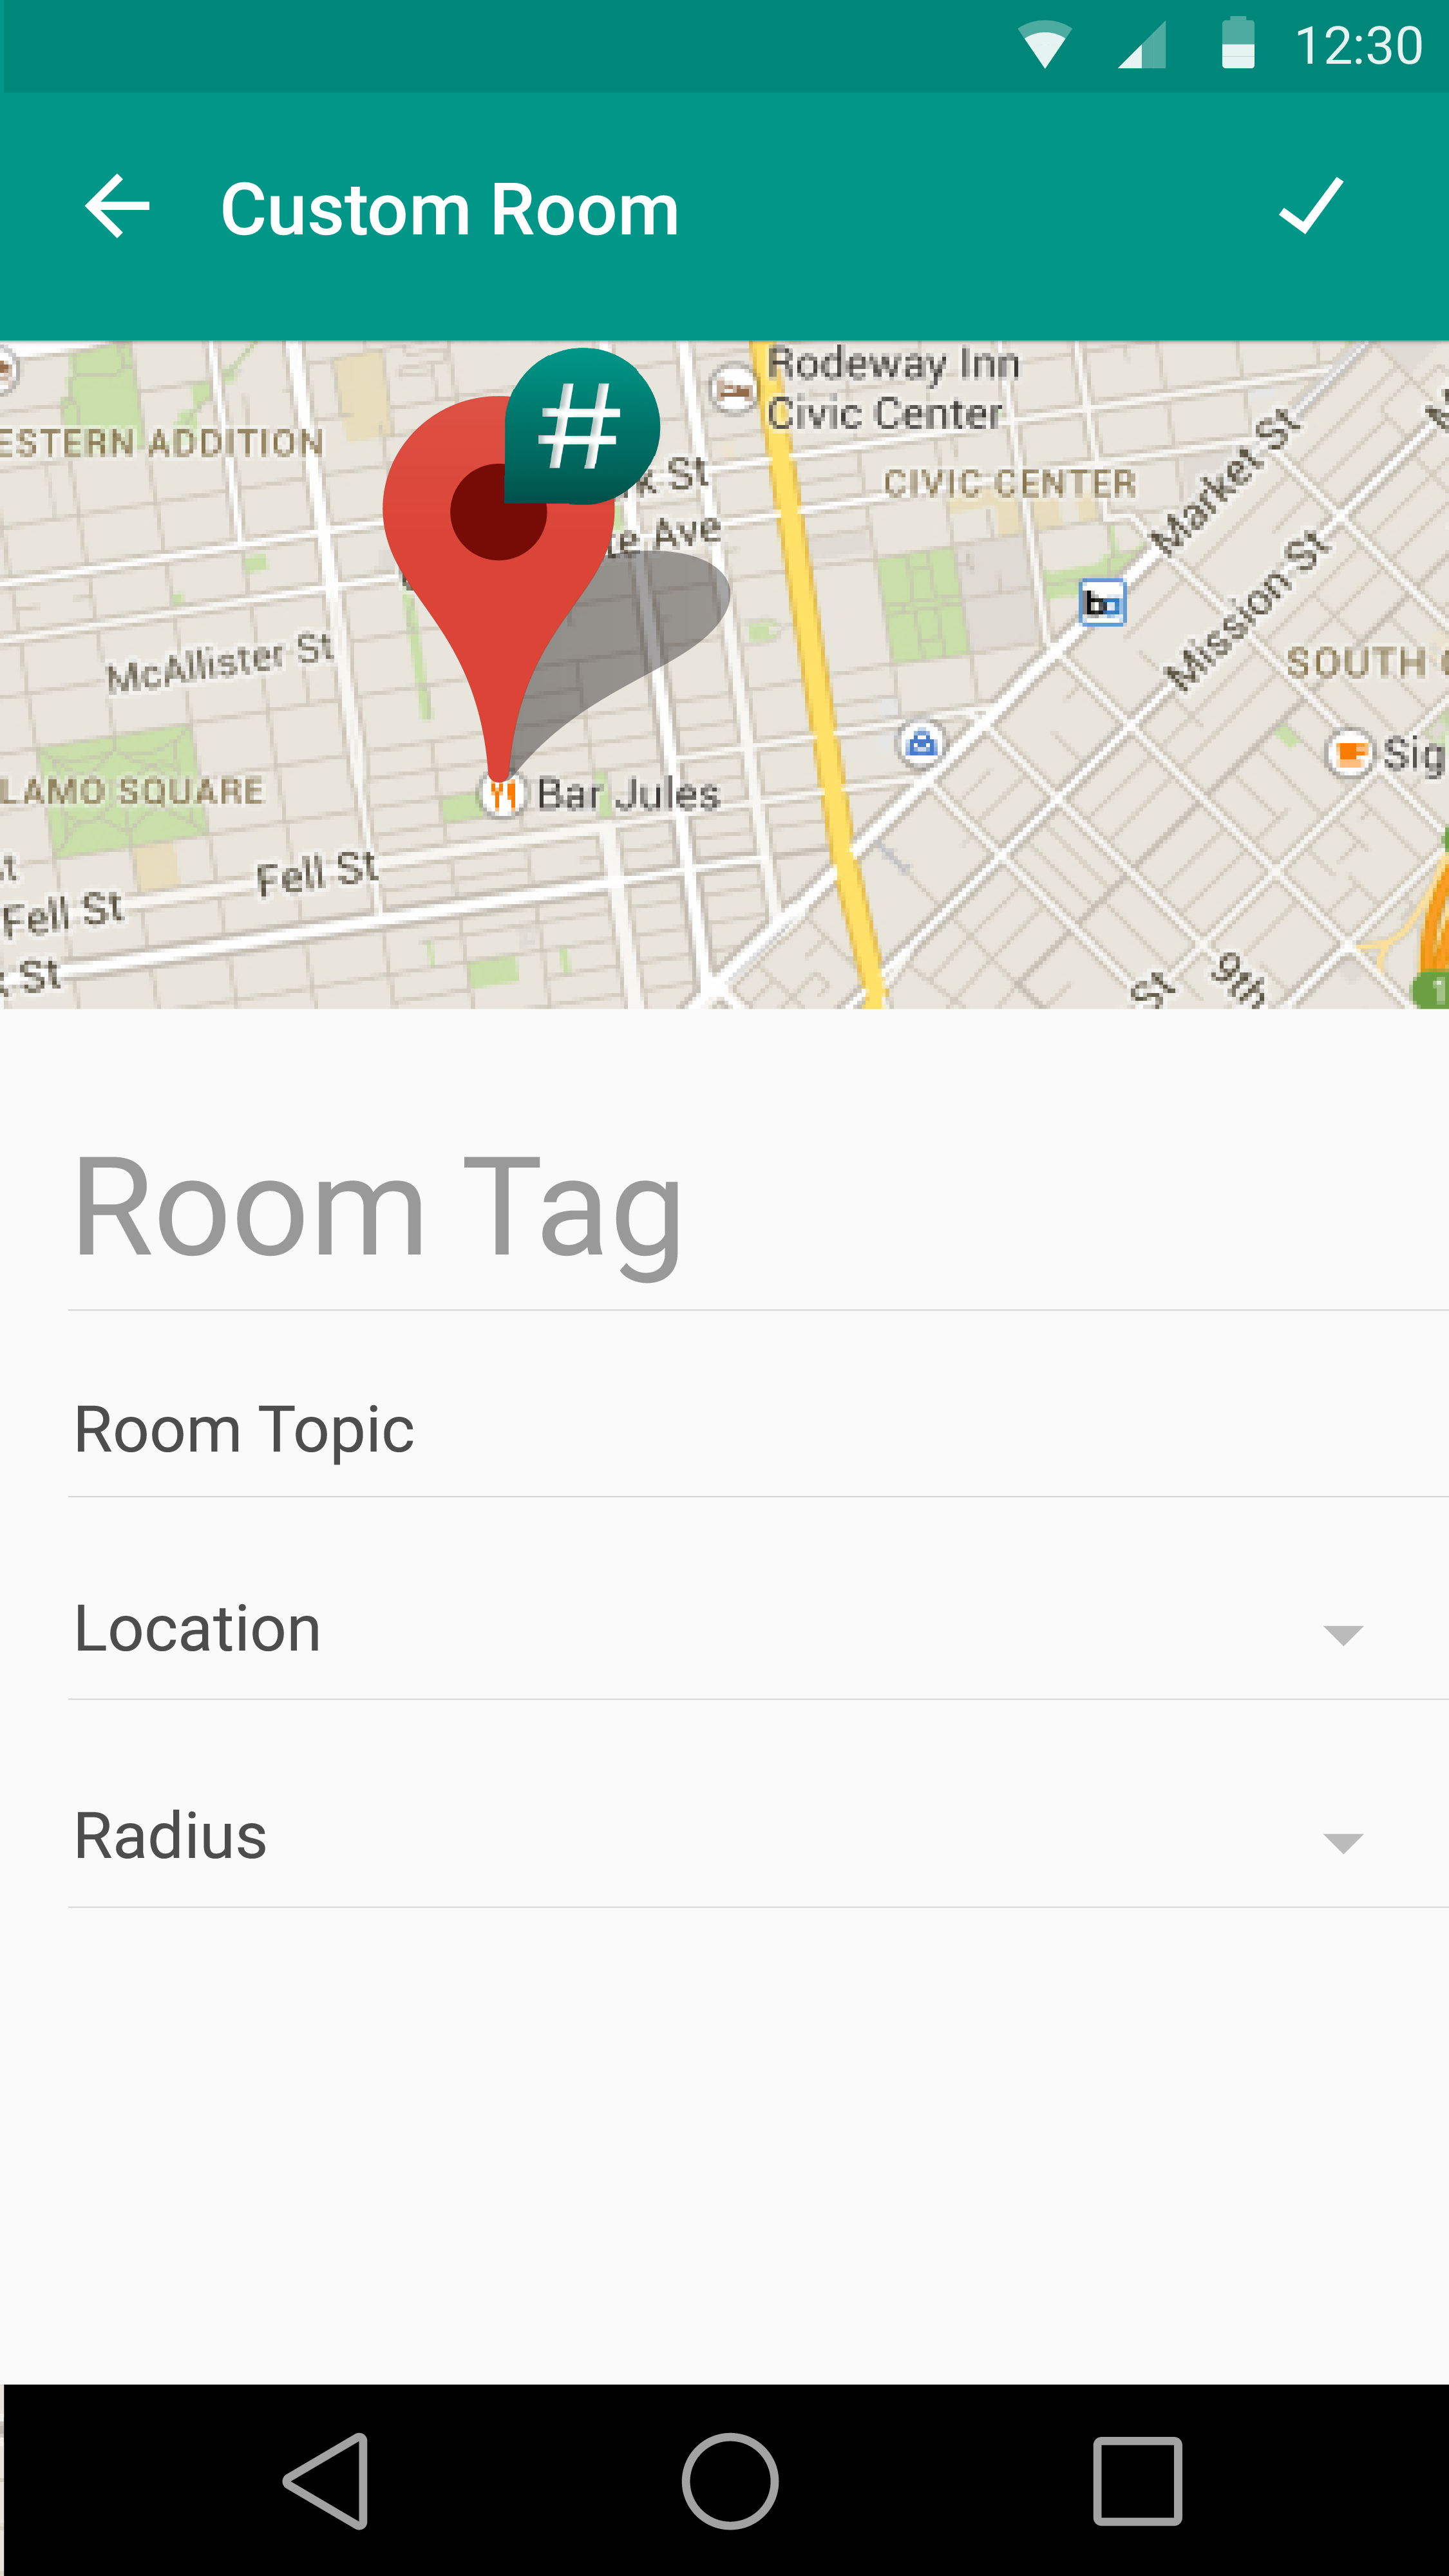
\includegraphics[width=5cm]{images/trendChattr_New_Room.png}}
    }\\
    \end{figure}
    \begin{figure}[H]
    \centering{
      \fbox{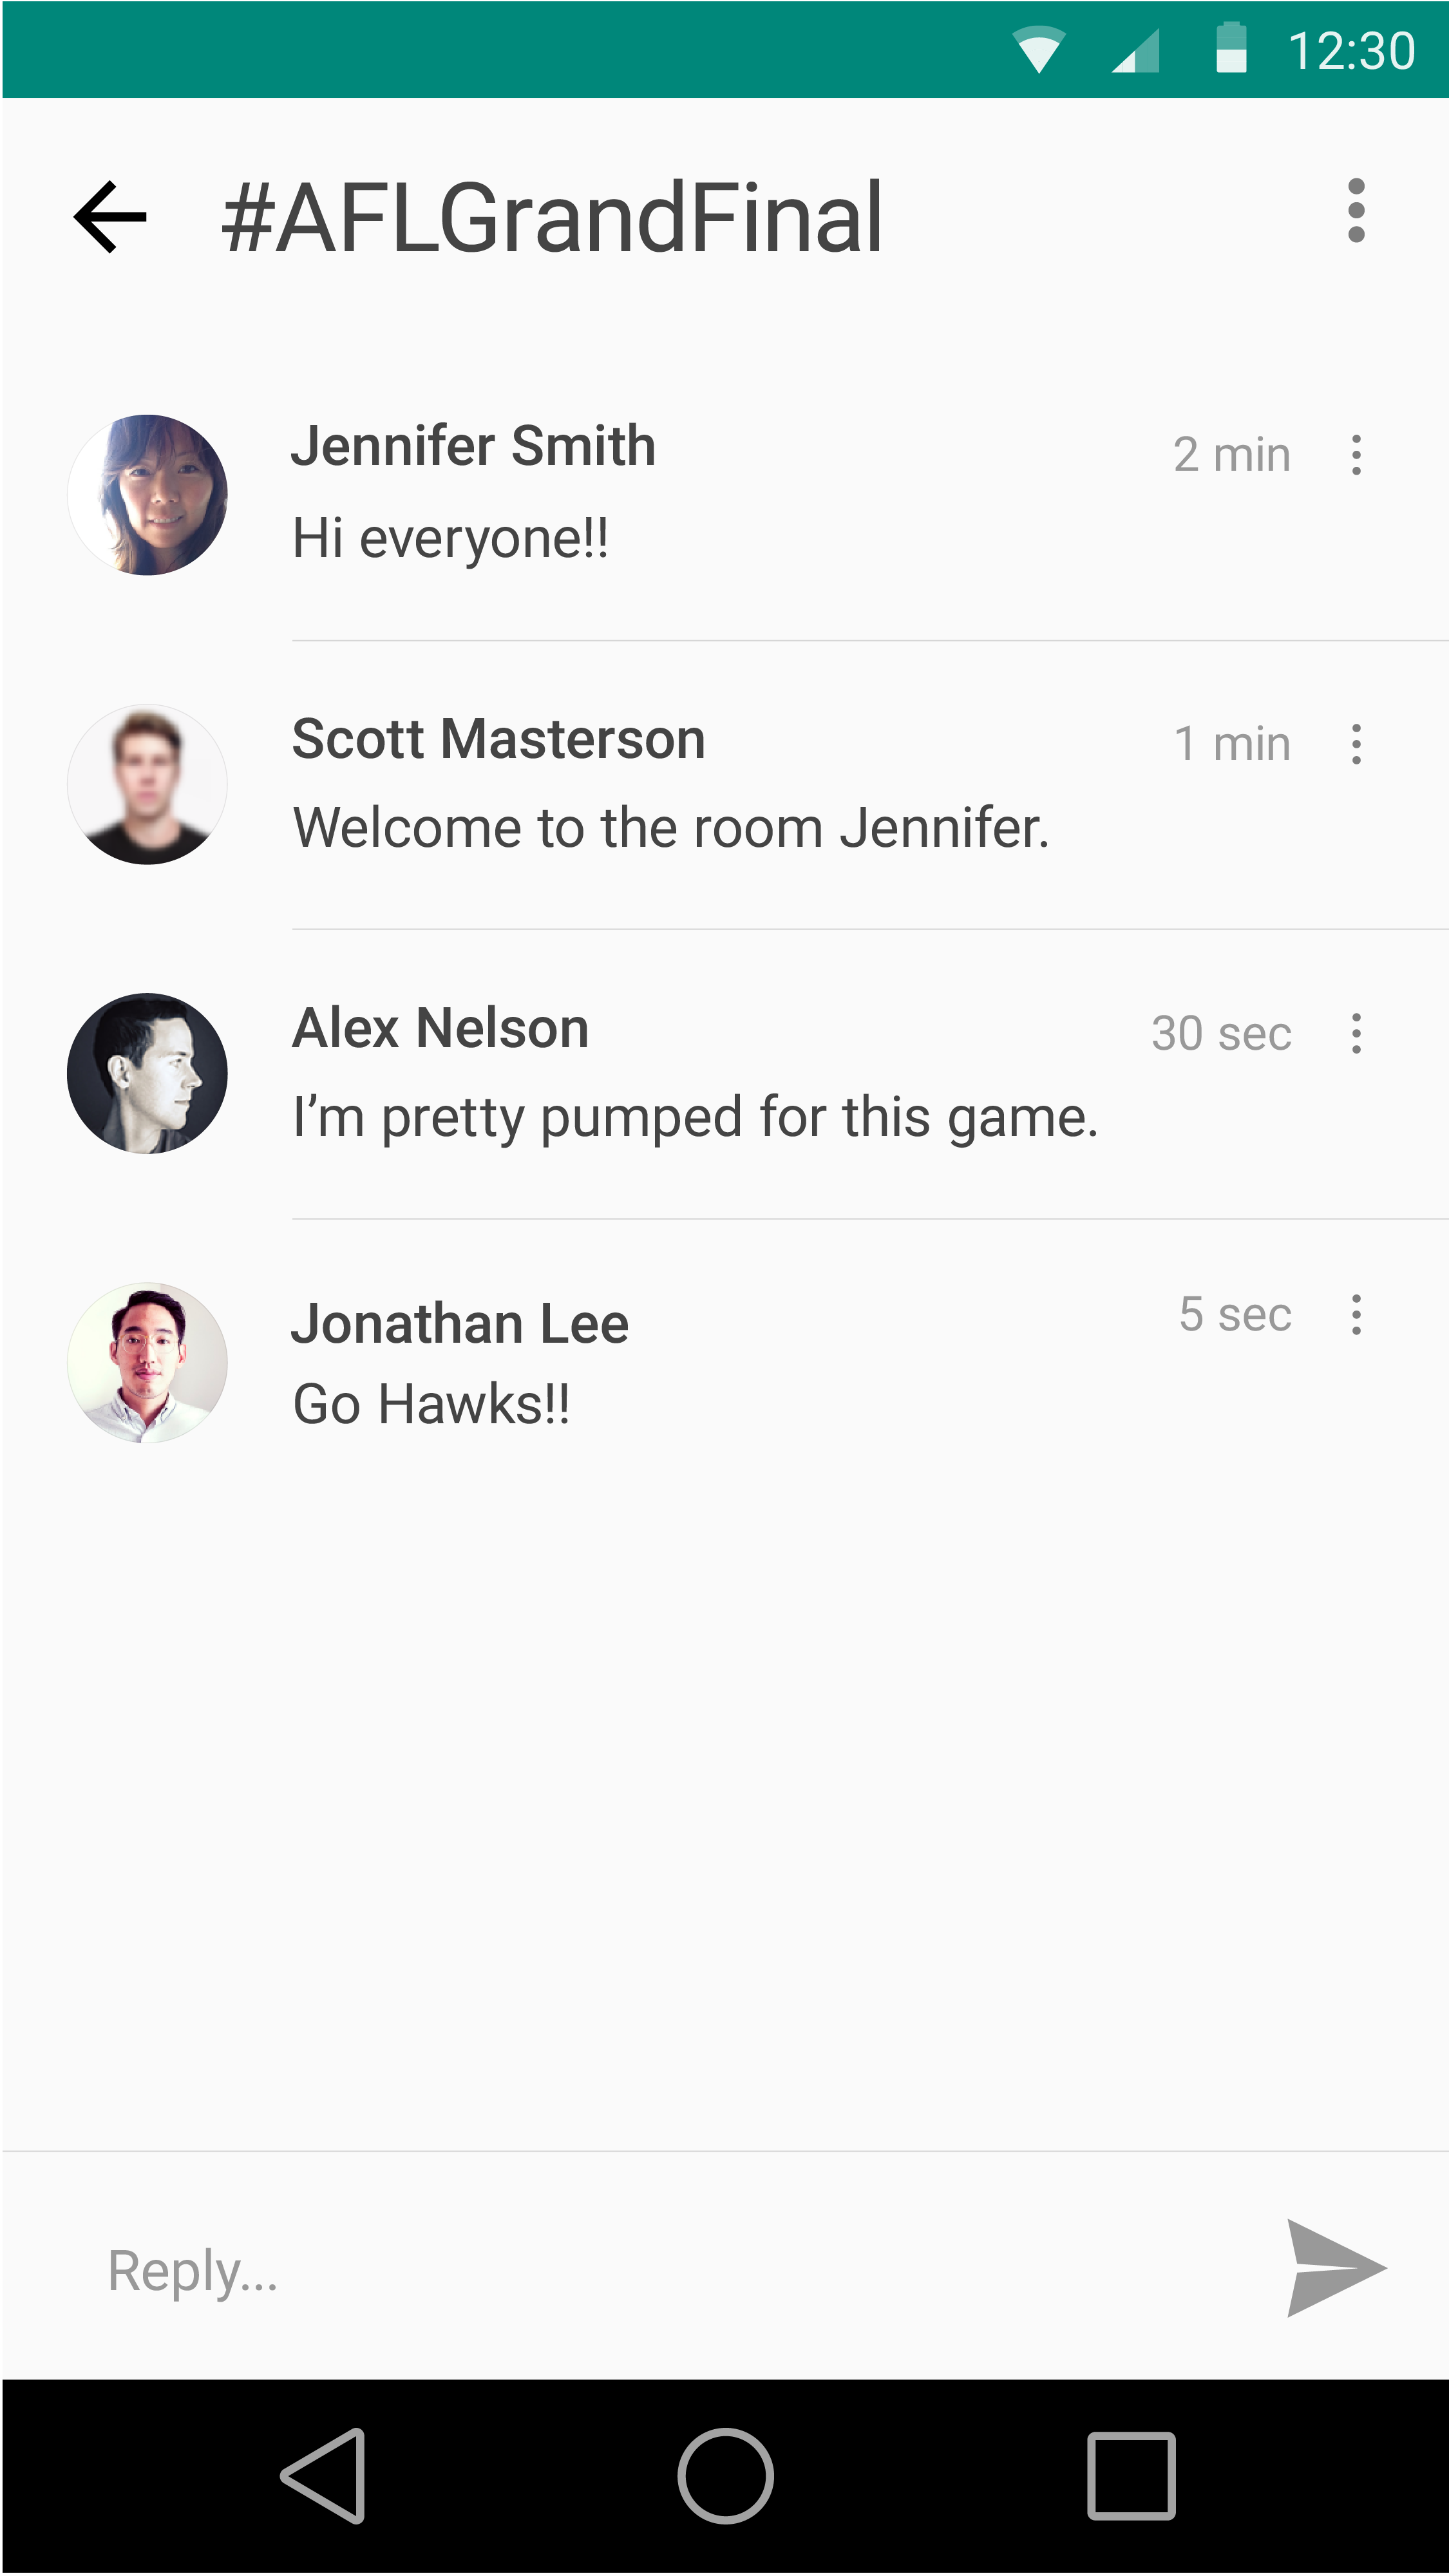
\includegraphics[width=5cm]{images/trendChattr_Chat_Window.png}}
    }\\
    \end{figure}

  \subsection{Questions}
    \begin{itemize}
      \item{Do the users link their accounts with twitter?}
    \end{itemize}

\end{document}
